\artikelfoto{Wiskundig programmeren in Python}{}{Dennis Presotto \\ Luc Van den Broeck}{img/LOEP/pythonbanner.jpeg}

\startcontents[inhoudloep]	% om inhoud voor het loep artikel te beginnen

\begin{multicols}{2}
	\inhoudstafelloep	
    %Om de layout van deze inhoudstafel te optimaliseren: pas \setcounter{tocdepth}{2} aan naar     \setcounter{tocdepth}{1} in de definitie van dit commando in uitwiskeling-style-sty
    % om inhoudstafel voor het loep artikel te tonen
	
	%% Gebruik \section{titel} en \subsection{titel} om genummerde tussentitels te maken
    \section{Inleiding}
    
    De informaticawereld staat niet stil. En in het onderwijs volgen wij haar op de voet. Na het tijdperk van de grafische zakrekenmachine hebben wij ons op apps en sofwarepakketten gefocust. Deze horde hebben we met plezier en met succes genomen. De volgende uitdaging staat nu met een beetje ongeduld aan de voordeur te trappelen: we laten onze leerlingen zelf programmeren. Heb je nog wat koudwatervrees voor de duik in dit onbekende water met diepe gronden? Dan kan deze loep je wellicht inspiratie bieden. 
    \vfill\null
    \columnbreak
    \subsection{Eindtermen en leerplannen}
    
    Er is bijzonder weinig informatie over een mogelijke brug tussen wiskunde en programmeren in de \emph{eindtermen} te vinden. Ook in de \emph{leerplannen} vinden we slechts karige suggesties. De leerplannen wiskunde verwijzen geregeld naar het gebruik van ICT voor berekeningen maar daarvoor hoeft er niet noodzakelijk geprogrammeerd te worden. Vaak volstaat GeoGebra (zie de loep van 39/4). 

    In de leerplannen informaticawetenschappen spreekt men over het oplossen van wiskundige problemen via numerieke methodes. Daarbij wordt verwezen naar nulwaarden, extrema, afgeleiden, integralen,  matrixvermenigvuldiging en stelsels. Maar ook hier volstaat het in eerste instantie om apps en softwarepakketten te gebruiken.
    
    In deze loep hebben we ervoor gekozen om rijen, reeksen, het benaderen van nulwaarden en `big data'-statistiek te behandelen. Dit zijn immers de onderwerpen waarvoor een programmeertaal een duidelijke meerwaarde biedt. 
    
    De eindtermen en leerplannen spreken zich niet uit over de te gebruiken programmeertaal. In deze loep hebben we gekozen voor Python omdat de auteurs hier voldoende ervaring mee hebben. Ook wordt Python in het hoger onderwijs vaak gebruikt en is de leercurve ervan niet te steil. Het spreekt voor zich dat de meeste idee\"en van deze loep eveneens in andere programmeertalen gebruikt kunnen worden.
	
    \subsection{Voor wie is deze loep?}
    
    We willen met deze loep aantonen hoe Python ingezet kan worden in functie van de lessen wiskunde, vooral bij studierichtingen in de derde graad met minstens 6 uren wiskunde. Enerzijds krijgen leerlingen in deze richtingen het vak informaticawetenschappen, anderzijds worden hier meer wiskundige onderwerpen gezien die zich lenen tot programmeren dan in richtingen met minder uren wiskunde. 
    
    Deze loep kan zowel interessant zijn voor leerkrachten wiskunde als voor leerkrachten informatica. Het aanleren van de programmeertaal Python zal grotendeels in een vak informaticawetenschappen gebeuren terwijl het aanleren van de wiskundige achtergrondkennis in het vak wiskunde gebeurt. De lesactiviteiten in deze loep kunnen aan de leerlingen voorgeschoteld worden in het vak wiskunde, in het vak informaticawetenschappen of in een project van co-teaching. Dat laatste biedt vermoedelijk het beste van beide werelden, al begrijpen we dat dit praktisch niet altijd haalbaar is. Vaak ook krijgt de leerkracht  wiskunde het vak informaticawetenschappen in zijn mandje gelegd.

   Deze loep richt zich op lezers met een beetje basiskennis van Python. We maken gebruik van lussen en van verschillende soorten datatypen, leerstof die ook in het vak informaticawetenschappen behandeld zal worden. Als je eerder weinig basiskennis van Python hebt, hoef je niet meteen te stoppen met lezen. In de programma's voegden we in groene tekst gebruikerscommentaar toe (voorafgegaan van een \#-teken). Die kan je al een eind op weg zetten.
   
   Je informaticacollega kan je waarschijnlijk ook goede sites of boeken aanraden. We hebben enkele suggesties toegevoegd in de bronnenlijst van dit artikel. Je kunt ook een kijkje nemen in de technische slotopmerkingen in paragraaf \ref{sec:technisch}.
	
    \subsection{Waarover gaat deze loep niet?} \label{sec:watniet}
    
    We focussen hier niet op de mogelijke manieren waarop de programmeertaal aangeleerd kan worden in het vak informaticawetenschappen.

    Deze loep gaat evenmin over de verwerking van grote datasets die opgenomen is in de eindtermen statistiek voor humane wetenschappen. Daar spreekt men expliciet over datasets van hooguit enkele honderden lijnen. Bij zulke, relatief kleine, datasets is het interessanter om GeoGebra of Excel te gebruiken.

    Tot slot geven we mee dat we vaak \'e\'en mogelijke code geven voor een bepaalde probleemstelling. Dit wil niet zeggen dat er geen alternatieve of zelfs effici\"entere programma's zijn. 
 
	
	\section{Rijen en reeksen}
        Bij de leerstof over rijen en reeksen beperken de eindtermen zich tot rekenkundige en meetkundige rijen en reeksen. Deze komen vaak voor in toepassingen en er zijn allerhande formules beschikbaar om bepaalde termen of reekssommen te berekenen. Bij rijen met andere recursieve voorschriften zijn de expliciete voorschriften vaak niet gekend en wordt het berekenen van een willekeurige term van de rij veel arbeidsintensiever. Op dat punt kan een Python-programma helpen bij de berekeningen. We geven hiervan enkele voorbeelden.

        \subsection{Eenvoudige recursieve voorschriften.}
        De volgende lesactiviteit focust op het al dan niet convergeren van rijen met recursieve voorschriften. 
        \end{multicols}
        \begin{lesactiviteit}{Termen berekenen bij rijen met een recursief voorschrift}
            Wanneer we kijken naar rijen die niet rekenkundig of meetkundig zijn, dan is het niet gemakkelijk om een expliciet voorschrift te vinden wanneer een recursief voorschrift gegeven is. Het handmatig berekenen van de termen van zo een rij door het herhaald gebruiken van een recursief voorschrift vraagt veel tijd. Python kan ons helpen bij het rekenwerk. \begin{vraagenantwoord}
            \vraag{Schrijf een Python-programma dat de achtste term berekent voor de volgende rij:
                $$u_1=2 \textrm{ en } u_{n+1}=\dfrac{1}{u_n^2}.$$
            Welke waarde krijg je voor $u_8$?}
            \antwoord{In het kader hieronder zie je een Python-programma met op elke regel een beetje gebruikerscommentaar na het \inline{#}-teken. Merk op dat we het recursief voorschrift zeven keer nodig hebben om van $u_1$ naar $u_8$ te gaan.
            \lstinputlisting[style=pythonstyle]{python/recursief1.py}
            We vinden $u_8 \approx 2,938 \cdot 10^{-39}$.}
            \vraag{Je zou kunnen denken dat de rij convergeert naar nul. Pas de code aan om de tussenliggende termen te tonen. Bevestigt dit je vermoeden dat deze rij convergeert?}
            \antwoord{Het volstaat om het printcommando op regel 4 te laten inspringen zodat het binnen de for-lus past. De rij divergeert, maar niet naar oneindig. We krijgen afwisselend zeer kleine en zeer grote getallen. Dat kun je ook zien aan het recursieve voorschrift: daar krijg je afwisselend zeer kleine en zeer grote getallen in de noemer.}
            \vraag{Laat Python nu de eerste tien termen van de volgende rij printen: 
            $$u_1=2 \textrm{ en } u_{n+1}=\dfrac{1}{1+u_n^2}.$$
            Convergeert deze rij?}
            \antwoord{
            De rij lijkt te convergeren naar een getal tussen $0,65$ en $0,7$. Let vooral op de insprong in de vijfde programmalijn.}
            \lstinputlisting[style=pythonstyle]{python/recursief2.py}
            \vraag{Pas de code zo aan dat de rij berekend wordt totdat het verschil tussen twee opeenvolgende termen hoogstens 0,001 is.}
            \antwoord{We gebruiken een while-lus in plaats van een for-lus. We vinden als limiet ongeveer $0,682$. In de vijfde regel van de code hebben we \inline{term+=verschil} gebruikt als afkorting voor \inline{term=term+verschil}.}\lstinputlisting[style=pythonstyle]{python/whileipvfor.py}
            \vraag{Kun je nu met zekerheid zeggen dat de rij convergeert?}
            \antwoord{De Python-code vormt geen formeel bewijs, maar ze geeft ons wel een sterk vermoeden van convergentie. Het lijkt erop dat de termen alternerend groter en kleiner zijn dan de vorige term. Ook lijkt het erop dat het verschil tussen twee termen alsmaar kleiner wordt.}
            \end{vraagenantwoord}
    
        \end{lesactiviteit}
        \begin{multicols}{2}
        Via deze eerste lesactiviteit zien de leerlingen dus het verschil tussen een print-commando binnen een lus of eentje erbuiten. Ze zien ook het verschil tussen de for-lus en de while-lus. De eerste heeft een vast aantal iteraties, de tweede werkt met een stopcriterium. We zullen later in de lesactiviteit van Newton-Raphson zien dat dit soms aanleiding kan geven tot oneindige lussen.

        Ook vanuit wiskundig standpunt valt er over deze lesactiviteit nog veel te zeggen. Zo is het kleiner worden van het verschil tussen twee termen geen voldoende voorwaarde voor de convergentie van de rij. Denk bijvoorbeeld aan de rij van partieelsommen van de harmonische reeks: $\displaystyle s_n = \sum_{i=1}^n \frac{1}{i}$. Daarbij geldt $\displaystyle \lim_{n \rightarrow \infty} (s_{n+1}-s_n)=0$ maar $\displaystyle \lim_{n \rightarrow \infty} s_n= + \infty$.

        De convergentie van de rij uit de bovenstaande lesactiviteit kan op twee manieren beargumenteerd worden. Enerzijds kun je deze convergentie grafisch inzien via een zogenaamde webgrafiek. Hierbij construeer je via de rechte met vergelijking $y=x$ en de grafiek van $f(x)=\dfrac{1}{1+x^2}$ alle koppels van de vorm $(x_n,f(x_n))=(x_n,x_{n+1})$. Het feit dat de rij convergeert, herken je aan de inwaartse spiraal die in dit geval ontstaat bij de webgrafiek. (Je kunt zelf webgrafieken maken via bijvoorbeeld de GeoGebra-applet van Wim Haazen: \url{https://www.geogebra.org/m/pEJYpjQ9}.)

        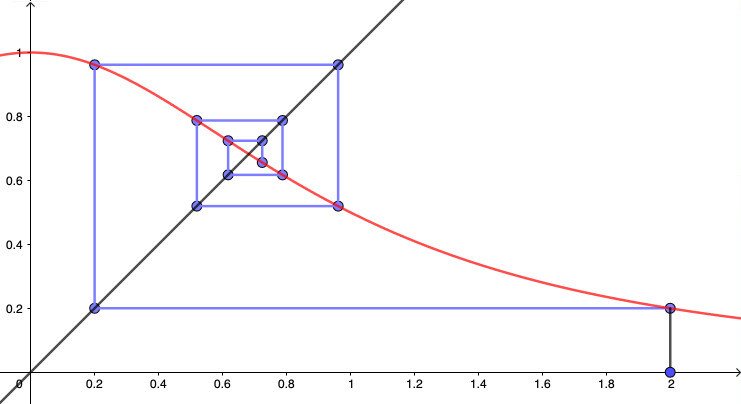
\includegraphics[width=0.45\textwidth]{img/LOEP/Webgrafiek.jpg}\\

        Anderzijds kan de convergentie ook algebra\"isch beargumenteerd worden: de rij convergeert naar het unieke fixpunt van de functie $f$. Dat laatste volgt uit het feit dat het beeld van $f$ gelijk is aan $]0,1]$ en uit het feit dat de beperking van $f$ tot het interval $[0,1]$ een zogenaamde (Lipschitz-)contractie is. We verwijzen naar (Labie \& Stulens, 2005) voor wie meer informatie wil over webgrafieken en stellingen in verband met fixpunten en iteratie.


        
        \subsection{De rij van Fibonacci}

        De rij van Fibonacci is een klassiek voorbeeld van een rij met een recursief voorschrift dat meer dan enkel de vorige term gebruikt. In de volgende lesactiviteit komen de leerlingen in aanraking met de datatypes \inline{list}, \inline{float} en \inline{int}. 
        \end{multicols}
        \begin{lesactiviteit}{De rij van Fibonacci}
        De rij van Fibonacci wordt gedefinieerd via een recursief voorschrift:
        $$ F_0=0, F_1=1 \textrm{ en } F_{n+1}=F_n+F_{n-1}.$$
        Elke nieuwe term wordt berekend op basis van de voorgaande twee. Voor de Python-code is het dus nodig dat er twee variabelen of een lijst gebruikt worden om die vorige twee termen van de rij te onthouden. De volgende opdrachten gaan hier verder op in.

        \begin{vraagenantwoord}
          \vraag{Je krijgt de volgende code voor het produceren van de getallen $F_0$, \ldots , $F_{10}$ van de Fibonacci-rij. Laat het programma lopen en ga na of je de juiste rij krijgt.}  

            \lstinputlisting[style=pythonstyle]{python/Fibonaccifout.py}
        \antwoord{Deze code produceert de rij $0, 1, 2, 4, 8, 16, 32, 64, 128, 256, 512$. Het programma berekent dus de eerstvolgende $9$ machten van $2$, niet de rij van Fibonacci.}
        \vraag{Welke fout werd er gemaakt in de code?}
        \antwoord{De variabele \inline{vorigeterm} (die staat voor $F_{n-1}$) wordt al overschreven door \inline{huidigeterm} alvorens we de vorige twee termen hebben opgeteld. Als gevolg daarvan tellen we altijd de laatste term op bij zichzelf en wordt de voorgaande term dus steeds verdubbeld.}
        \vraag{Hoe kun je de code aanpassen om toch de juiste termen $F_0, \ldots, F_{10}$ van de Fibonacci-rij te krijgen?}
        \antwoord{Optie 1: We voeren een hulpvariabele in.}
        \lstinputlisting[style=pythonstyle]{python/Fibonacci1.py}
        
        \antwoord{Optie 2: We veranderen de waarden van de variabelen \inline{huidigeterm} en \inline{vorigeterm} in eenzelfde stap.}
        \lstinputlisting[style=pythonstyle]{python/Fibonacci2.py}
            
        \antwoord{Optie 3: We slaan alle getallen op in een lijst en printen die pas op het einde. Merk op dat de range van de lus nu tot $11$ loopt. Dat komt doordat twee iteraties van de lus nodig zijn om de getallen $0$ en $1$ toe te voegen aan de lijst.}
        \lstinputlisting[style=pythonstyle]{python/Fibonacci3.py}
        
        \antwoord{Optie 4: Een verkorte aanpak met een lijst. We starten met de waarden $0$ en $1$ in de lijst zodat er twee iteraties minder nodig zijn van de lus. Ook vermijden we het gebruik van de variabelen \inline{a} en \inline{b}.}
        \lstinputlisting[style=pythonstyle]{python/Fibonacci4.py}

        Een van deze vier opties werd geschreven door AI, daarover later meer. Heb jij alvast door welke optie niet van menselijke makelij is?
        
        \vraag{Voor de Fibonacci-rij is een expliciet voorschrift gekend (de formule van Binet):
            $$ F_n = \frac{\left(\frac{1+\sqrt{5}}{2}\right)^n - \left(\frac{1-\sqrt{5}}{2}\right)^n}{\sqrt{5}}.$$ Schrijf een Python-code die dit expliciet voorschrift gebruikt om $F_0$, \ldots , $F_{10}$ te berekenen. 
            }
        \antwoord{Voor de vierkantswortel moeten we de library `\inline{math}' importeren.}
        \lstinputlisting[style=pythonstyle]{python/Fibonacciexact1.py}

            
            \vraag{Als je dit programma laat lopen, dan ziet het antwoord er een beetje vreemd uit. Verklaar wat er gebeurt en pas je code aan.}
            \antwoord{We krijgen als output. \begin{align*}
            & 1.0 \\
            & 2.0 \\
            & \vdots \\
            & 55.000000000000014
            \end{align*}
            Python is bij het berekenen van de vierkantswortels overgegaan op datatype \inline{float} in plaats van \inline{integer}. We kunnen dit oplossen door de laatste regel van de code aan te passen naar \inline{print(round(getal))}. Zo houden we ook rekening met de afrondingsfouten die Python maakt bij het berekenen van vierkantswortels gezien hier slechts eindig veel decimalen in rekening gebracht worden.}
        \end{vraagenantwoord}
        \end{lesactiviteit}
        \begin{multicols}{2}
        We geven tot slot nog mee dat het aantonen van dit expliciete voorschrift van de rij van Fibonacci een mooie oefening op inductiebewijzen is. We focussen in deze loep echter vooral op Python en gaan niet dieper in op dat bewijs. Een voorbeeld van dit bewijs is te vinden op \url{https://www.cut-the-knot.org/proofs/BinetFormula.shtml}.
        \subsection{Reekssommen berekenen}
        Tot slot kijken we naar reeksen. Ook hier beperken de meeste cursussen zich tot rekenkundige en meetkundige reeksen omdat het bij andere reeksen vaak moeilijk is om convergentie aan te tonen of formules te vinden voor de partieelsommen. Het vinden van de limiet van een convergerende reeks is niet altijd makkelijk. De volgende lesopdracht behandelt een bekend voorbeeld voor het benaderen van $\pi$. Deze lesactiviteit kan gebruikt worden als verdere toepassing op lussen maar ook op de verkorte schrijfwijze \inline{+=}, \inline{-=}, \ldots

        \end{multicols}
        \begin{lesactiviteit}{Werken met reeksen}
        Eén van de eerste gekende (reeks)formules voor $\pi$ is van de hand van de Indische wiskunde Madhava. In de veertiende eeuw ontdekte hij de volgende gelijkheid voor een hoek $\theta$ in radialen:
        $$ \theta = \tan(\theta) - \frac{\tan^3(\theta)}{3} + \frac{\tan^5(\theta)}{5} - \frac{\tan^7(\theta)}{7} + \ldots $$
        Wanneer we $\theta$ gelijk stellen aan $\frac{\pi}{4}$, dan krijgen we
        $$ \frac{\pi}{4} = 1 - \frac{1}{3} + \frac{1}{5} - \frac{1}{7} + \ldots $$
        of nog
        $$ \pi = 4 - \frac{4}{3} + \frac{4}{5} - \frac{4}{7} + \ldots $$
        \begin{vraagenantwoord}
            \vraag{Hoeveel termen heb je in deze reeks nodig om $\pi$ tot op 0,001 nauwkeurig te bepalen?}
            \antwoord{Aangezien we een alternerende reeks hebben waarvan de termen in absolute waarde dalen en naar nul convergeren, weten we zeker dat de $n$-de partieelsom $s_n$ nauwkeurig genoeg is, wanneer de absolute waarde van de $(n+1)$-de term kleiner is dan $0,001$. Op onderstaande tekening wil dat zeggen dat de afstand tussen de limiet $s$ en de partieelsom $s_n$ hoogstens $0,001$ is wanneer $b_{n+1} =  |s_{n+1}-s_n|$ hoogstens $0,001$ is. De limiet $s$ ligt immers tussen deze twee partieelsommen in. Voor het huidige voorbeeld is $b_n = \dfrac{4}{2n+1}$.
            \begin{center}
               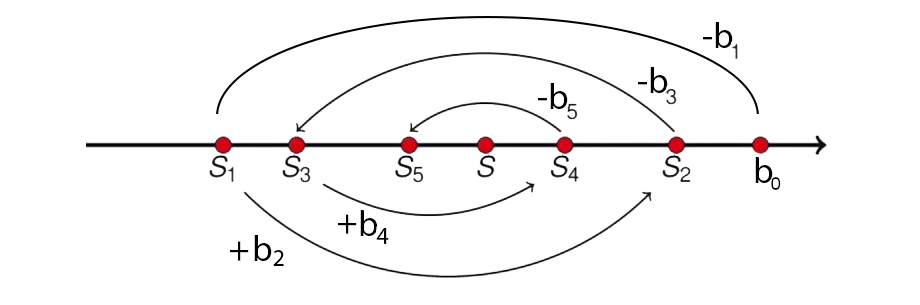
\includegraphics[width=0.5\textwidth]{img/LOEP/Alternating2.jpg} \\
               (afbeelding gebaseerd op \url{https://www.youtube.com/watch?v=j1VlpaNBkkA})
            \end{center}
            Voor deze reeks vinden we
            \begin{align*}
                \frac{4}{2(n+1)+1} &< 0,001 \\
                & \Updownarrow \\
                n & \geqslant 1999
            \end{align*}
            We hebben de som van de eerste $2000$ termen van de reeks nodig, want de eerst term is $b_0$ en de laatste is $b_{1999}$.
            }
\clearpage
           \vraag{Bereken deze partieelsom via een Python-programma. Gebruik daarbij de verkorte schrijfwijze \inline{+=} in je berekening.}
           \antwoord{Via de volgende code vinden we als benadering $3,14109265$. }
            \lstinputlisting[style=pythonstyle]{python/benaderpi.py}
        \end{vraagenantwoord}
        \end{lesactiviteit}
        \begin{multicols}{2}
        Deze lesactiviteit over de benadering van $\pi$ kan wiskundig verder uitgediept worden. Zo valt het waarschijnlijk op dat er erg veel termen nodig zijn om slechts 3 beduidende cijfers te vinden. Dat komt doordat de gegeven reeks erg traag convergeert. Het kan daarom nuttig zijn om dit te vergelijken met andere reeksen die sneller convergeren en waar dus minder termen nodig zijn voor 3 beduidende cijfers. (Zie bijvoorbeeld de pagina `Approximations of $\pi$' op \url{wikiwand.com}.)
        
	
	%\begin{kader}{Kadertype}{Titel van dit kader}
	%	\lipsum[1][1-2]
	%\end{kader}

	\section{Benaderen van nulwaarden}
        Veel handboeken staan vol met oefeningen waarbij het mogelijk is om met de hand de nulwaarden van de gegeven veeltermfuncties, rationale functies, \ldots te vinden. In realistische voorbeelden gebeurt het echter vaak dat de nulwaarden niet geheel zijn zodat de methode van Horner (of een andere exacte methode) niet toegepast kan worden en enkel een benadering mogelijk is. Meestal wordt hiervoor een grafiek getekend met ICT waarbij dan de snijpunten met de $x$-as bij benadering afgelezen worden. Als toepassing op afgeleiden of op de stelling van Bolzano is het echter interessant om numerieke benaderingen te behandelen.
        
        \subsection{Methodes zonder als-dan-structuur}
        De bekendste methode voor het benaderen van de nulwaarden van een functie is vermoedelijk de methode van Newton-Raphson. Deze methode is gebaseerd op het volgende centrale idee: wanneer we de nulwaarde van een functie benaderen door een bepaalde $x$-waarde en voor deze $x$-waarde de raaklijn tekenen aan de grafiek van de functie, dan is de nulwaarde van de eerstegraadsfunctie die de raaklijn beschrijft meestal een betere benadering van de nulwaarde van de functie dan de $x$-waarde waarvan we vertrokken zijn. Deze constructie genereert dus een rij van alsmaar betere benaderingen voor de nulwaarde van de functie. Visueel ziet dit er als volgt uit.

        \begin{center}
        \includegraphics[width=0.45\textwidth]{img/LOEP/Newtonraphson.png}
        \captionof{figure}{Benadering van het nulpunt met de methode van Newton-Raphson}
        \end{center}
        
        Het is eenvoudig om de leerlingen te laten inzien dat deze constructie het volgende recursief voorschrift voor de achtereenvolgende benaderingen geeft:
        $$x_{n+1} = x_n - \frac{f(x_n)}{f'(x_n)}.$$ In de volgende lesactiviteit gebruiken we deze methode om de nulwaarde van een derdegraadsfunctie te zoeken.

        

        \end{multicols}
        \begin{lesactiviteit}{De methode van Newton-Raphson}
        We gaan op zoek naar de nulwaarde(n) van de veeltermfunctie $f$ met als voorschrift:
        $$f(x) = x^3 -2x -2.$$
        \begin{vraagenantwoord}
            \vraag{Stel het verloopschema van $f$ op om na te gaan dat $f$ maar \'e\'en nulwaarde heeft.}
            \antwoord{We vinden als afgeleide $f'(x)=3x^2-2$. Dit levert ons het volgende verloopschema:\\
            \begin{center}
             \begin{tabular}{c|ccccccc}
                $x$ & $-\infty$ & & $-\sqrt{\dfrac{2}{3}}$ & & $\sqrt{\dfrac{2}{3}}$ & & $+\infty$ \\
                \hline
               $f'(x)$  & & + & $0$ & $-$ & $0$ & + & \\
               \hline
               $f(x)$ & & $\nearrow$ & $\overset{rel}{max}$ & $\searrow$ & $\overset{rel}{min}$ & $\nearrow$ & \\
            \end{tabular}
            \end{center}
            Omdat $f\left( -\sqrt{\dfrac23}\right) = \dfrac43 \sqrt{\dfrac23} - 2 < 0 $ weten we dat er slechts \'e\'en nulwaarde is. Die nulwaarde is bovendien groter dan $\sqrt{\dfrac23}$.
            }
            \vraag{Ga na dat $f$ geen gehele nulwaarden heeft zodat we niet kunnen verderwerken met de methode van Horner.}
            \antwoord{Uit het verloopschema weten we al dat de nulwaarde positief moet zijn. We proberen de natuurlijke delers van de constante term als mogelijke nulwaarden. Gezien $f$ gehele co\"effici\"enten heeft, zijn dit de enige kanshebbers voor gehele nulwaarden. We vinden:
            $$ f(1)=-3\neq 0 \textrm{ en } f(2)=2 \neq 0.$$}
            \vraag{Leg uit waarom deze berekening je wel informatie geeft over de waarde van de nulwaarde van $f$.}
            \antwoord{Omdat $f$ continu is en  $f(1)$ en $f(2)$ tegengestelde tekens hebben, moet er een nulwaarde zijn in het interval $]1,2[$ (wegens de tussenwaardestelling of de stelling van Bolzano).}
            \vraag{Wat is bijgevolg een goede startwaarde voor de methode van Newton-Raphson?}
            \antwoord{Een mogelijk startpunt is het midden van het interval, dus $x_0 = 1,5$. In het algemeen kun je deze keuze ook laten afhangen van het feit of de grafiek hol of bol is en van de functiewaarden in de randpunten van het interval.}
            \vraag{Schrijf nu een Python-code die Newton-Raphson uitvoert tot het verschil tussen twee opeenvolgende benaderingen kleiner is dan 0,0001.}
           \antwoord{In dit programma moeten $f(x)$ en $f'(x)$ verschillende keren berekend worden. We defini\"eren daarom functies in Python die dit berekenen. Dat doen we via het commando \inline{def}. We vinden dat de nulwaarde ongeveer gelijk is aan $1,7693$.}

           \lstinputlisting[style=pythonstyle]{python/NewtonRaphson.py}
            \vraag{Wat gebeurt er wanneer je ditzelfde programma laat starten bij de waarde $x_0=0$?}
            \antwoord{We krijgen een Timeout-melding. Python is in een oneindige lus beland.}
            \vraag{Kun je deze Timeout-melding verklaren? Doe dit zowel numeriek als grafisch.}
            \antwoord{\begin{multicols}{2}
            We kunnen met de hand narekenen dat de benaderingen in de volgende oneindige lus terecht komen: $$x_0=0, x_1=-1, x_2=0, x_3=-1, \ldots$$ 
            Met Python zouden we dit kunnen zien door de while-lus te vervangen door een for-lus waarbij we het aantal iteraties op voorhand vastleggen. We kunnen de oneindige lus ook grafisch zien: de raaklijn aan de grafiek van $f$ in het punt $(0,f(0))$ snijdt de $x$-as in $(-1,0)$ en de raaklijn aan $f$ in het punt $(-1,f(-1))$ snijdt de $x$-as in $(0,0)$.
            \columnbreak
            \includegraphics[width=0.27\textwidth]{img/LOEP/NewtonRaphsononeindig.png}
            \end{multicols}}
        \end{vraagenantwoord}
        Uiteraard kun je veel van die oneindige lussen vermijden door de startwaarde voldoende dicht bij de nulwaarde te kiezen. Toch zijn er ook functies waarbij Newton-Raphson nooit naar de nulwaarde zal convergeren (bijvoorbeeld $f(x) = \sqrt[3]{x^3-2x-2}$). Om zulke problemen met oneindige lussen te vermijden kun je een safestop inbouwen. In de bovenstaande code kan dit door een extra variabele \inline{stap} in te voeren die onthoudt hoeveel keer de lus al doorlopen is:\\
            \lstinputlisting[style=pythonstyle]{python/NewtonRaphsonsafe.py}

        Dit programma vertelt ons ook dat de benadering 1,7693 gevonden werd na 3 stappen.
        \end{lesactiviteit}

    \begin{multicols}{2}
    Ter informatie geven we mee dat de functie \inline{str} in de laatste regel van de vorige lesactiviteit gebruikt werd om aan Python duidelijk te maken dat we een aaneenschakeling van verschillende strings willen en geen optelling wanneer we het symbool $+$ gebruiken.
    \subsection{Methodes met als-dan-structuur}
    Naast éénpuntsmethodes zoals Newton-Raphson bestaan er ook meerpuntsmethodes om nulwaarden te bepalen. We behandelen hier twee voorbeelden waarbij convergentie gegarandeerd is, maar waarbij als-dan-constructies (dus if-statements) nodig zijn bij implementatie in Python.\\

    \end{multicols}

    \begin{lesactiviteit}{De middelpuntsmethode van Bolzano}
        
        De stelling van Bolzano zegt dat wanneer een functie continu is op een gesloten interval $[a,b]$ en $f(a)$ en $f(b)$ een verschillend teken hebben, de functie $f$ een nulwaarde heeft in het interval $]a,b[$. Dit wordt meestal bewezen door een rij deelintervallen te maken via het volgende principe. Splits het interval in twee even grote helften $[a,m]$ en $[m,b]$ en ga vervolgens verder met het interval waarvan de grenswaarden beeldwaarden met een verschillend teken hebben. Door dit proces te itereren, krijgen we een alsmaar kleiner interval.

        Gebruik deze methode om een interval van breedte hooguit 0,001 te cre\"eren dat de nulwaarde bevat van de functie $f$ met als voorschrift:
        $$f(x) = \ln(x)+x.$$
        \begin{vraagenantwoord}   
            \vraag{Verklaar waarom $f$ exact \'e\'en nulwaarde heeft.}
            \antwoord{$f$ is een (strikt) stijgende functie met $\displaystyle \lim_{\underset{>}{x \rightarrow 0}}f(x) = - \infty$ en $\displaystyle \lim_{x \rightarrow + \infty}f(x) = + \infty$}        
            \vraag{Geef een interval (van eindige lengte) dat deze unieke nulwaarde met zekerheid bevat.}
           \antwoord{ $f(1)=0+1>0$. We zoeken dus nog een getal met negatieve functiewaarde. We zoeken zo een getal tussen $0$ en $1$ en vinden bijvoorbeeld $f\left( \dfrac{1}{e} \right) = -1 + \dfrac{1}{e} < 0.$ De nulwaarde ligt dus met zekerheid in het interval $\left]\dfrac{1}{e},1\right[.$}
            \vraag{Schrijf een Python-programma dat deze nulwaarde benadert door het interval te blijven halveren in lengte tot je een interval van breedte hooguit 0,001 hebt.}
           \antwoord{
            We vinden dat de nulwaarde ligt tussen $0,5666$ en $0,5673$. Voor het gevalsonderscheid hebben we een \inline{if}-commando gebruikt. Merk in de laatste regel op dat we + gebruiken in plaats van , om de strings aan elkaar te plakken. Dit is om te vermijden dat er een spatie geprint wordt in het interval.}

            \lstinputlisting[style=pythonstyle]{python/Bolzano.py}
            
            \vraag{Bereken hoeveel stappen Python nodig had om deze benadering te vinden.}
            \antwoord{De breedte van het interval halveert bij elke stap. De breedte van het startinterval was $1-\dfrac1e$. Zodoende voldoet de gezochte $n$ aan
            \begin{align*}
                \frac{1-\frac{1}{e}}{2^n} &\leqslant 0,001 \\
                & \Updownarrow \\
                n & \geqslant {}^2\log\left(\frac{1-\frac{1}{e}}{0,001}\right) \approx 9,3
            \end{align*}
            Er waren dus $10$ stappen nodig.
            }
            \vraag{Hoe kun je dit aantal stappen controleren via Python?}
            \antwoord{Je definieert een variabele \inline{stap=0} vóór het begin van de while-lus. Binnen de while-lus laat je die teller met 1 toenemen via de regel \inline{stap+=1}. Op het einde van de code vraag je om ook de variabele \inline{stap} te printen. We zien dat die inderdaad de waarde $10$ had.}
        \end{vraagenantwoord}
    \end{lesactiviteit}



     \begin{lesactiviteit}{De regula-falsi-methode}
        Analoog aan de middelpuntsmethode van Bolzano vertrekt de methode van regula-falsi vanuit een interval $[a,b]$ waarbij $f(a)$ en $f(b)$ verschillende tekens hebben. Dit interval wordt opnieuw opgesplitst in kleinere intervallen, ditmaal gebaseerd op het snijpunt van de rechte door $(a,f(a))$ en $(b,f(b))$ met de $x$-as. Gebruik deze methode om de nulwaarde van 
        $f$ met als voorschrift:
        $$f(x) = \ln(x)+x$$
        te vinden in het interval $\left]\dfrac{1}{e},1\right[$.

        \begin{vraagenantwoord}  
            \vraag{Ga na dat de rechte door $(a,f(a))$ en $(b,f(b))$ de $x$-as snijdt in het punt met $x$-co\"ordinaat $x=\dfrac{af(b)-bf(a)}{f(b)-f(a)}$.}
            \antwoord{Deze rechte heeft als vergelijking
            $$ y-f(a) = \dfrac{f(b)-f(a)}{b-a}(x-a)$$
            en de nulwaarde daarvan is $$x=a - \dfrac{b-a}{f(b)-f(a)}\cdot f(a) =  \dfrac{af(b)-bf(a)}{f(b)-f(a)}.$$}
            \vraag{Kun je verklaren waarom het stopcriterium \inline{while b-a>0.001} niet zal werken bij een Python-programma voor regula-falsi? Hint: teken enkele stappen van deze methode op de grafiek.}
            \begin{multicols}{2}
            \antwoord{Bij de regula-falsi-methode convergeert slechts \'e\'en van de grenswaarden van het interval naar de nulwaarde. Welke grenswaarde dit is, hangt af van de tekens van $f(a)$ en $f(b)$ en van het feit of de grafiek hol of bol is in de omgeving van de nulwaarde. Voor de functie van de grafiek hiernaast zien we dat enkel de rechtergrens van het interval naar de nulwaarde zal convergeren. Het verschil $b_i-a_i$ gaat niet naar nul.   
            \columnbreak
            \includegraphics[width=0.3\textwidth]{img/LOEP/RegulaFalsiGrenspunt2.png}}
            \end{multicols}
            
            \vraag{Geef een alternatief stopcriterium dat wel zou werken voor deze methode.}
            \antwoord{We kunnen de lus laten stoppen zodra $f(m)$ klein genoeg is, waarbij $m = \dfrac{af(b)-bf(a)}{f(b)-f(a)}$.}
            \vraag{Benader de nulwaarde van de gegeven functie met behulp van de regula-falsi-methode waarbij je stopt wanneer $f(m)$ kleiner is dan 0,001.}
            \antwoord{We vinden dat de nulwaarde bij benadering $0,567$ is. Voor de leesbaarheid van het programma voeren we functies in voor de berekening van $m$ en $f(m)$.}
            \lstinputlisting[style=pythonstyle]{python/RegulaFalsi.py}
        \end{vraagenantwoord}
        \end{lesactiviteit}

        \begin{multicols}{2}
        
        Qua wiskundige toevoeging geven we mee dat de convergentie van één van de randpunten van regula-falsi verloopt via de monotone convergentiestelling. De ondergrenzen vormen bijvoorbeeld een stijgende rij die nooit boven de initi\"ele bovengrens van het eerste interval kan gaan. Zodra bewezen is dat de rij ondergrenzen en rij bovengrenzen convergeren, kan via een bewijs vanuit het ongerijmde aangetoond worden dat een van deze rijen naar de nulwaarde convergeert.


    \subsection{Iteratief programmeren versus recursief programmeren}
    In alle bovenstaande voorbeelden hebben we ervoor gekozen om te werken met for-lussen of while-lussen. Dit wordt ook wel eens iteratief programmeren genoemd. Binnen zo een lus wordt een bepaalde bewerking immers herhaald of ge\"itereerd. Hier bestaat echter een alternatief voor: recursief programmeren. Bij recursief programmeren werk je via functies die (onder bepaalde voorwaarden) zichzelf terug oproepen maar dan met andere startwaarden. 
    
    Hieronder zie je een voorbeeld van hoe het voorbeeld van de regula-falsi-methode eruit zou zien met recursief programmeren. Merk daarbij op dat de functie regulafalsi zichzelf oproept in regels 17 en 19.
    \end{multicols}
            \lstinputlisting[style=pythonstyle]{python/RegulaFalsirecursief.py}

    \begin{multicols}{2}



\section{Big data}
    Big data zijn niet meer weg te denken uit onze maatschappij. Er worden (openlijk of verdoken) data verzameld over ons aankoop- en surfgedrag, over ons energieverbruik, onze verplaatsingen ... Het is dan ook logisch dat de verwerking van big data mondjesmaat in onze lessen infiltreert.
    
    In deze paragraaf beschrijven we hoe Python ingezet kan worden om datasets te analyseren die te groot of te onhandig zijn voor Excel of GeoGebra. We leggen hier uit hoe je in Python kunt werken met csv-bestanden (comma separated values), hoe je histogrammen kunt maken van geselecteerde gegevens uit deze bestanden, hoe je gemiddelden en standaardafwijkingen kunt berekenen en hoe je de normaliteit van de bepaalde gegevens kunt controleren. Maar we kijken vooral naar de interpretatie van deze aspecten van de databestanden. De datasets en ook de programma's die we voor de lesactiviteiten gebruiken, vind je terug op de website van Uitwiskeling. 
    
    In tegenstelling tot de bovenstaande paragrafen zijn hier vaak extra commando's nodig die niet in de basiskennis van de meeste leerlingen en leerkrachten zitten. Er komen ook specifiekere  packages aan bod dan bijvoorbeeld het veelgebruikte `\inline{numpy}'. Daarom hanteren we hier een stijl waarbij de code niet door de leerlingen zelf geschreven moet worden maar waarbij ze aangereikte codes interpreteren en deze naar eigen behoefte aanpassen.

\subsection{Werken met csv-datasets}

    Als inleiding op een diepgaander onderzoek naar grote datasets werpen we eerst een blik op het type van het csv-bestand.

    In een csv-bestand worden data (getallen, datums, tekst, booleans ...) zonder enige opmaak gestockeerd. Elke rij bevat alle gegevens van een bepaalde identiteit (persoon, voertuig, dag, ...), telkens in dezelfde volgorde. Csv is niet alleen een zuinig formaat om digitale data te verzenden maar het is ook een formaat dat compatibel is met heel wat softwaretoepassingen. 
    
    De volgende lesactiviteiten zouden de leerlingen ervan moeten overtuigen dat het kijken naar de getallen in een csv-bestand op zich weinig inzicht oplevert. De data moeten dus op een andere manier verwerkt en geanalyseerd worden. 
    
    Csv-bestanden verwerken in GeoGebra of in Excel heeft beperkingen als het gaat over zeer grote bestanden. Daarom gaat de voorkeur van data-analysten vaak uit naar een analyse met Python (of naar het gebruik van professionele statistische software zoals R, SPSS en SAS). 

\end{multicols}
\begin{lesactiviteit}{Csv-bestanden}
    
    Een csv-bestand (comma separated values-bestand) is een bestand waarin gegevens zonder opmaak regel per regel bewaard worden. Tussen twee opeenvolgende waarden staat een komma (of een puntkomma of een tab-teken) als scheidingsteken (separator). Tussen twee opeenvolgende regels staat een end-of-line-teken. De meeste softwaretoepassingen aanvaarden csv-bestanden als input. We onderzoeken hier hoe we een csv-bestand het makkelijkst kunnen bekijken en de inhoud ervan kunnen analyseren.

\lestitel{Aantallen bevallingen per dag}
    Sinds 1 januari 1992 hield het Belgisch nationaal bureau voor statistiek, vroeger het NIS en nu StatBel, dagelijks gegevens bij over de geboortes in België. We bezorgen je een bestand `\inline{geboortesperdag.csv}' waarin het aantal bevallingen per dag is opgenomen. Het zou een interessante activiteit kunnen zijn te onderzoeken of er geboortepieken zijn, of het aantal geboortes stelselmatig in de tijd toe- of afneemt, of de geboortes seizoensgebonden zijn enz.

    \begin{vraagenantwoord}
		
    
    \vraag{Open het csv-bestand in  Excel en beschrijf wat je in dit bestand ziet. Beschrijf zowel de vorm als de inhoud. Verklaar ook waarom je de gegevens op deze manier ziet.}
		
    \antwoord{We zien een tabel met \num{10958} rijen waarin voor elke rij naast elkaar een datum staat, een dagnaam en een aantal geboortes. Elke rij stelt een waarneming uit onze dataset voor. De waarnemingen zijn niet in de meest gebruiksvriendelijke vorm weergegeven: alles staat in de meest linkse kolom (zie onderstaande figuur links). Dat is de standaardinstelling als je op een csv-bestand klikt om het in Excel te openen maar het is niet de meest gebruiksvriendelijke. Om deze data makkelijk te kunnen analyseren, moeten we de gegevens over verschillende kolommen vepreiden (zie onderstaande figuur rechts). Je kunt dit doen door in Excel de separator `komma' in te stellen via de gegevenswizard (gegevens > uit tekstbestand/csv). De gegevens zijn nu overzichtelijker gepresenteerd maar het grote aantal rijen in het dataframe blijft het overzicht belemmeren. Er zijn talrijke mogelijkheden in Excel om selecties in het rekenblad te maken en hier analyses op te doen. Je zult echter af en toe door lange tabellen moeten scrollen en het is sowieso lastig om te zien of je de juiste blokken hebt geselecteerd in deze tabellen. Foutjes zijn hier snel gemaakt.}
    \begin{minipage}[t]{0.5\linewidth}
            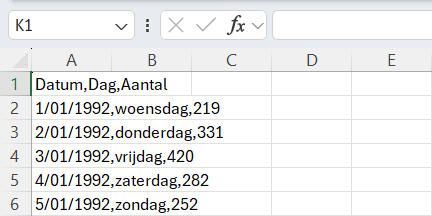
\includegraphics[width=6cm]{img/LOEP/excelGeboorten.jpg}
        \end{minipage}\hfill
        \begin{minipage}[t]{0.5\linewidth}
            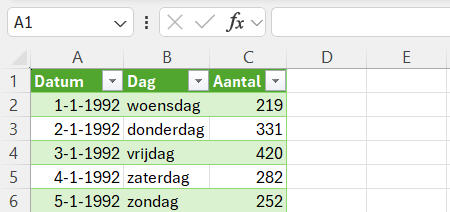
\includegraphics[width=6.5cm]{img/LOEP/excelGeboorten2.jpg}
        \end{minipage}
		
    \vraag{Kun je de gegevens ook in een rekenblad van GeoGebra invoeren?}

    \antwoord{Met knippen en plakken kun je gegevens overzetten van Excel naar GeoGebra, als dit programma je voorkeur geniet. De gegevens komen netjes in verschillende kolommen terecht. Maar als je enkele duizenden gegevens wil verwerken, loopt het systeem vast. GeoGebra is niet ontwikkeld voor big data.}
		
    \end{vraagenantwoord}

    Een interessantere manier om big data te analyseren en te manipuleren is via Python. Python beschikt over een \emph{package} (een module of een bibliotheekprogramma) dat verregaande statistische analyses kan uitvoeren: `\inline{pandas}'. Deze module moet eerst geladen worden. Daarna kan Python csv-bestanden lezen en ze omzetten naar een \inline{dataframe}.



    \begin{vraagenantwoord}[resume]
    
    \vraag{Maak een pythonbestand met de volgende inhoud en bewaar het in een map waarin ook \inline{geboortesperdag.csv} zit. Op deze manier kan het Python-programma het csv-bestand makkelijk vinden. Verklaar alle programmaregels.}
        
    \lstinputlisting[style=pythonstyle]{python/csvAantalGeboortesPerDag.py}

    
    \antwoord{In regel 4 wordt Pandas geïmporteerd. Verderop zal er naar Pandas verwezen worden met de afkorting \inline{pd}. Als we een functie uit Pandas willen gebruiken, noteren we deze functie achter de modulenaam, gescheiden door een punt. Zo wordt in regel 9 de functie \inline{read_csv} uit Pandas gebruikt om een csv-bestand te lezen.}

    \vraag{Laat het programma lopen en beschrijf wat je ziet.}
    \afbeelding[7cm]{img/LOEP/csvGeboorten.jpg}{}{geboorten}
    \antwoord{Hierboven zie je dat een dataframe een automatische nummering in de linkerkolom heeft die begint bij $0$. Er zijn \num{10958} rijen. De kolommen in een dataframe hebben een titel die aangeeft wat er in elke kolom staat. Alleen de eerste en de laatste vijf rijen worden getoond. De rest is verborgen achter de stippeltjes. Kijken naar deze output leert je niet veel. Om meer zicht te krijgen op de situatie kan er bijvoorbeeld ook een grafische voorstelling gemaakt worden.}
    \end{vraagenantwoord}
\end{lesactiviteit}
\begin{multicols}{2}

\subsection{Grafische voorstellingen}
Om een duidelijker zicht te krijgen op een overvloed aan data kunnen we een grafische voorstelling maken zoals een spreidingsdiagram, een histogram en een boxplot.

De Pythonmodule `\inline{matplotlib}' zorgt voor deze grafische voorstellingen maar ze kan nog veel meer. We beperken ons in deze loep tot twee voorbeelden en een bescheiden interpretatie van de grafische output. 

Verderop zullen we de grafische interpretaties wiskundig ondersteunen door het berekenen van kengetallen, het toevoegen van trendlijnen en het opvragen van QQ-plots.

\end{multicols}
\begin{lesactiviteit}{Frequentiediagrammen}
    
   Bij een groot aantal opmetingen is het handig om de data in klassen te verdelen. We kunnen de klassen uitzetten op de horizontale as van een assenstelsel. Een diagram met staafjes/rechthoekjes met als basis de klassen en als oppervlakte de frequentie van deze klassen noemen we een \emph{histogram}. Als de frequentie niet de oppervlakte van de staafjes/rechthoekjes is maar wel de hoogte van de staafjes/rechthoekjes dan spreken we van een \emph{frequentiediagram}. 

   Om een frequentiediagram in Python te tekenen, hebben we de module \inline{matplotlib} nodig, meer bepaald de functie \inline{pyplot} uit deze module. \inline{matplotlib} is niet secuur bij de naamgeving van de diagrammen: frequentiediagrammen worden gemaakt met de instructie \inline{hist}.

    \lestitel{Aantallen geboortes per dag}
    We keren even terug naar het csv-bestand `\inline{geboortesperdag.csv}'. 

    \begin{vraagenantwoord}
    \vraag{Vul het vorige pythonbestand aan zoals hieronder aangegeven. Verklaar de programmaregels die erbij gekomen zijn.} 


    \lstinputlisting[style=pythonstyle]{python/Aantalgeboortesperdag1.py}
    
    \antwoord{In regel 4 wordt de functie \inline{pyplot} uit de module \inline{matplotlib} geïmporteerd. Ze wordt afgekort tot \inline{plt}. In regel 16 maken we een frequentiediagram van de kolom \inline{'Aantal'} uit het dataframe \inline{geboortes}. Het bestaat uit $50$ staafjes (Eng: bins) binnen het interval $[150,500]$. De volgende regels spreken voor zich. Er wordt een titel toegevoegd aan het frequentiediagram en de twee assen worden voorzien van een verklarende tekst. Een frequentiediagram opstellen is niet hetzelfde als een frequentiediagram afbeelden. Zonder de vermelding van regel 20 wordt er niets op het scherm getoond.}

    \vraag{Laat het Python-programma lopen. Hoe groot is de klassenbreedte? Hoeveel toppen heeft het frequentiediagram? Kun je hier een verklaring voor bedenken?}

    \antwoord{Bij het antwoord op vraag 4 zie je het frequentiediagram van de dagelijkse aantallen geboortes in België met klassenbreedte \emph{\(7\)}. Dit komt door het bereik (\(500-150\) door het aantal klassen (\(50\)) te delen. Verder is de verdeling bimodaal. Dit betekent dat het frequentiediagram een kamelencurve is: eentje met twee toppen. De laagste top zit rond de $215$ geboortes en hoogste rond de $375$ geboortes. Zou het verschil tussen week- en weekenddagen hier een rol in spelen? Of tussen feestdagen en gewone dagen? Dit zullen we verderop nog onderzoeken.}



    \vraag{Hoe zou je het verschil in de hoogte van de toppen kunnen verklaren}
    \antwoord{Als de toppen verklaard worden door het onderscheid tussen week- en weekenddagen dan wordt het verschil in hoogte verklaard doordat er meer weekdagen zijn dan weekenddagen.}

    \vraag{Hoe pas je dit frequentiediagram aan zo dat de gegevens niet in klassen gegroepeerd zijn?}

    \antwoord{Door een kleine wijziging in regel 16 wordt er één staafje per eenheid voorzien: bins=$350$. Merk op dat je dit laatste frequentiediagram nu ook een histogram mag noemen. De frequenties zijn zowel af te lezen van de hoogte als van de oppervlaktes van de staafjes (met breedte \emph{\(1\)}).\\
    \begin{minipage}[t]{0.5\linewidth}
        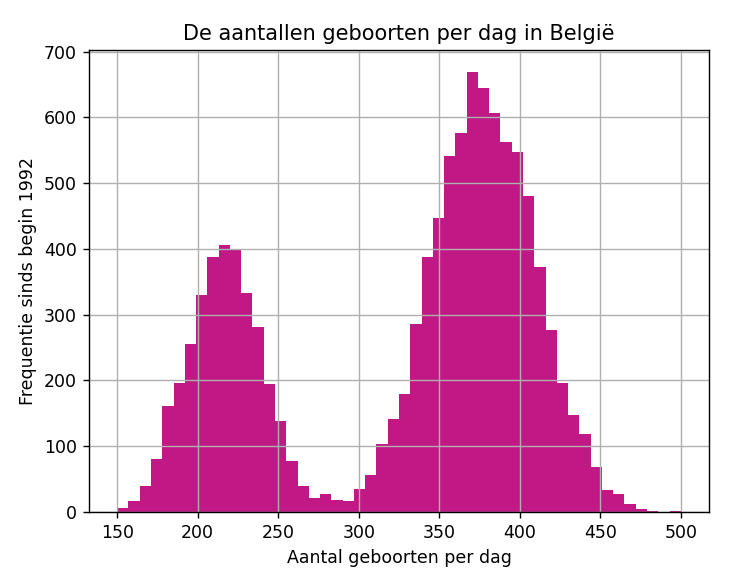
\includegraphics[width=6cm]{img/LOEP/histogramgeboorten1.jpg}
    \end{minipage}\hfill
    \begin{minipage}[t]{0.5\linewidth}
        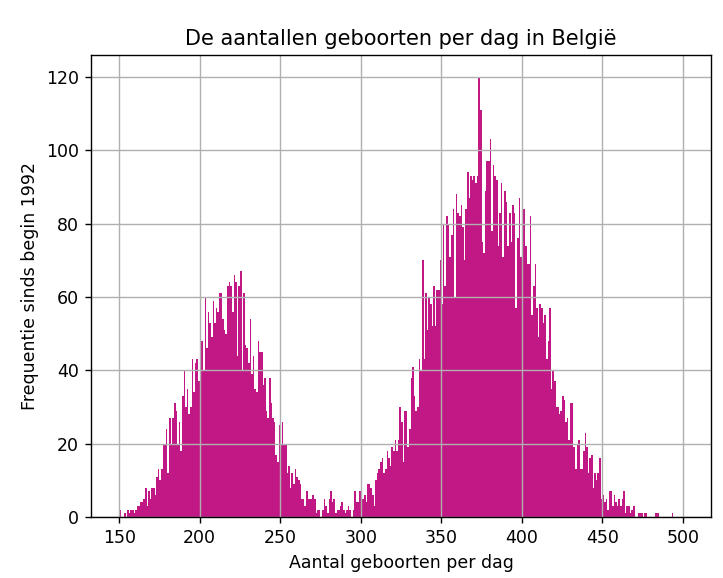
\includegraphics[width=6cm]{img/LOEP/histogramgeboorten2.jpg}
    \end{minipage}
    }
  \end{vraagenantwoord} 
\end{lesactiviteit}
\begin{multicols}{2}

In een tweede voorbeeld laten we zien hoe we een spreidingsdiagram maken. De begrippen \emph{spreidingsdiagram} en \emph{trendlijn} zijn gekend uit de tweede graad (zie UW 38/1: Spreidingsdiagrammen \& trendlijnen in de 2de graad).  

De leerlingen weten al dat de vorm van de puntenwolk ons iets leert over het verband tussen de twee grootheden. Als de stippen sterk gebundeld zijn rond een rechte, dan ligt de correlatiecoëfficiënt tussen de twee grootheden in de buurt van $1$ of van $-1$. Als de puntenwolk diffuus is dan ligt de correlatiecoëfficiënt dicht bij 0. 

Maar er zijn mogelijk nog andere besluiten te trekken uit de vorm van een puntenwolk. Een puntenwolk kan een periodisch verloop hebben, ze kan zich ook tegen een horizontale asymptoot aanleggen, soms kan ze benaderd worden door de grafiek van een exponentiële functie ... We illustreren de interpretatie van een spreidingsdiagram met een klasactiviteit in verband met sterftecijfers in België.
\end{multicols}

\begin{lesactiviteit}{Spreidingsdiagrammen}
    
   In de vorige lesactiviteit visualiseerden we een aantal meetwaarden met een histogram. In deze lesactiviteit visualiseren we \emph{koppels} van meetwaarden in een \emph{spreidingsdiagram}. Hierin wordt elk koppel van meetwaarden voorgesteld door een stip in een assenstelsel. De stippen samen vormen een puntenwolk. In deze lesactiviteit maken we een spreidingsdiagram van het dagelijkse aantal overlijdens in België. Op de horizontale as zetten we het dagnummer uit sinds het begin van de meting, op de verticale as zetten we het aantal overlijdens op de overeenkomstige dagen uit.

\lestitel{Sterftecijfers in België}
   Sinds 1992 houdt StatBel (het Belgisch statistisch bureau dat gegevens verzamelt over de bevolking, de economie, de infrastructuur en de landbouw in België) het dagelijkse aantal sterfgevallen in België bij. Dat zijn tot op heden \num{11323} gegevens. We willen nagaan of het dagelijkse aantal overlijdens sindsdien nagenoeg stabiel gebleven is. 
   
   De sterftecijfers worden ter beschikking gesteld via het bestand `\inline{overlijdensperdag.csv}'. Je kunt (bijvoorbeeld via Excel, Kladblok of Word) nagaan dat het scheidingsteken in dit bestand een kommapunt is. 

    \begin{vraagenantwoord}
    \vraag{Neem de volgende programmaregels over in Python en verklaar wat nieuw is.} 
    
    \lstinputlisting[style=pythonstyle]{python/steftecijfersperdag.py}
    
    \antwoord{In regel 5 wordt de module \inline{numpy} geïntroduceerd. Python biedt naast de vier basisbewerkingen weinig mogelijkheden om te rekenen. De module \inline{numpy} staat in voor alle mogelijke numerieke operaties: het berekenen van sinussen, van $n$-de-machtswortels en logaritmen, het werken met lijsten (arrays) ... Een toepassing van \inline{numpy} vind je in regel 20.\\
    Met \inline{np.arange(0, 12000, step=2000)} stellen we een rekenkundige rij op van getallen tussen 0 en \num{12000} met een verschil van \num{2000}. Deze rij wordt gebruikt om markeringen aan te brengen op de $x$-as. Bij het lezen van het csv-bestand in regel 11 moet er expliciet aangegeven worden dat de separator een puntkomma is. En tot slot: het spreidingsdiagram wordt opgesteld in regel 17. De \inline{markers} zijn puntjes met puntgrootte 2. Het diagram wordt getoond door regel 22.}

    \vraag{Laat het Python-programma lopen en interpreteer het resultaat zo goed mogelijk.}
    \antwoord{De grafiek hieronder maakt een cyclische beweging met $31$ toppen en $31$ dalen. Wellicht heeft dit te maken met een jaarlijkse cyclische beweging: veel sterfte in de winter, weinig sterfte in de zomer.}
    
    \afbeelding[10cm]{img/LOEP/overlijdens.jpg}{}{sterfte}
     
    \vraag{Aan de rechterkant van de grafiek zien we enkele uitzonderlijk hoge waarden. Kun je deze verklaren?}
    
    \antwoord{De hogen pieken komen overeen met de jaartallen \emph{2020} en \emph{2021} waarbij de oversterfte te wijten is aan de coronapandemie.}
    \vraag{De globale tendens is licht stijgend. Kun je dit verklaren?}
    \antwoord{Deze stijging is waarschijnlijk te verklaren door de aangroei van de Belgische bevolking maar ook door de dicht bevolkte generatie die momenteel door de vergrijzingszone schuift en die voor veel overlijdens zorgt.}
    \end{vraagenantwoord}
\end{lesactiviteit}


\clearpage
    
    \afbeelding[14cm]{img/statistiek-zoo.jpg}{}{}

\begin{multicols}{2}


\subsection{Gemiddelden, standaardafwijkingen en regressielijnen}

In de volgende lesactiviteit berekenen we kengetallen als het gemiddelde en de standaardafwijking en leggen we  tendensen bloot met regessielijnen. We stellen hiervoor een bestand ter beschikking met metereologische gegevens opgemeten in de stad Antwerpen. Deze dataset biedt talrijke mogelijkheden tot een dieper onderzoek in de klas. 

\end{multicols}
\begin{lesactiviteit}{Gemiddelde, standaardafwijking en regressielijn}
    
   Kijken naar een grafische voorstelling van big data is een begin. Maar hier houdt het natuurlijk niet op. In deze lesactiviteit willen we te weten komen of de opwarming van het klimaat in België werkelijk te zien is in de metingen. Ook willen we een voorspelling van de gemiddelde dagtemperatuur naar de toekomst doen. Daarom berekenen we eerst de kengetallen van een open-meteo-dataset en benaderen we de bijbehorende puntenwolk met een best passende grafiek.

    \lestitel{Gemiddelde dagtemperatuur}
    Via open-meteo.com kun je makkelijk metereologische metingen opvragen van verschillende plaatsen in België, voor de temperatuur zelfs van uur tot uur sinds het jaar 1940. Dat kan bestanden opleveren van bijna een miljoen regels. Zulke bestanden zijn moeilijk te hanteren via een spreadsheetsoftware. In het gedeelde bestand `\inline{openmeteoantwerpen.csv}' vind je metingen uit Antwerpen van alle dagen sinds 1940. Dit geeft een bestand van meer dan $30\,000$ regels. 

    \begin{vraagenantwoord}
    \vraag{Neem de volgende pythoncode over. Verklaar voor jezelf alle regels van dit programma.} 

   \lstinputlisting[style=pythonstyle,linerange={1-21},firstnumber=1]{python/meteo3.py}
    
    \antwoord{In dit programma komen drie nieuwe items voor: \inline{mean()} staat voor het gemiddelde, \inline{std()} staat voor de standaardafwijking en \inline{\\n} staat voor de overgang naar een nieuwe afdrukregel. In het bestand `\inline{openmeteoantwerpen.csv}' staan nog veel meer gegevens dan de gemiddelde dagtemperatuur. Ook windsnelheden, regen- en sneeuwval, opkomst en ondergang van de zon ... worden bijgehouden in dit bestand.}
    
    \vraag{Laat het programma lopen en vat samen wat je te zien krijgt.} 
    \antwoord{Het gemiddelde van de dagtemperaturen over meer dan $80$ jaar blijkt $10,38^\circ C$ te zijn en de standaardafwijking is $6,43^\circ C$. Deze twee getallen zeggen niets over de evolutie door de jaren heen. Willen we ons daarover uitspreken, dan moeten we een regressielijn berekenen. Dit komt onmiddellijk hierna aan bod. Als we de gemiddelde dagtemperatuur uit de vorige eeuw vergelijken met die van deze eeuw moeten we delen uit een dataframe kunnen selecteren. Dit komt verderop nog aan bod.}
    \end{vraagenantwoord}

    \lestitel{Puntenwolk en regressielijn}

    De puntenwolk die aan het csv-bestand \inline{openmeteoantwerpen.csv} gekoppeld is, lijkt min of meer periodisch. Dat zie je duidelijk op de figuur hieronder. De jaarlijkse cyclus verbaast uiteraard niet.

    \afbeelding[10cm]{img/LOEP/gemiddeldedagtemperatuur.jpg}{}{dagtemp}
    
    In plaats van de puntenwolk samen te vatten in twee getallen (gemiddelde en standaardafwijking) kunnen we ze ook samenvatten met een grafiek die een langjarige tendens laat zien die geen rekening houdt met uitschieters in zomer en winter. Statistici omschrijven dit als een weergave die ontdaan is van `ruis'. Deze grafiek zorgt ervoor dat we enkel focussen op de essentie. De blauwe rechte bovenop de puntenwolk in de figuur hieronder geeft een langjarige tendens weer. We noemen deze rechte een \emph{regressielijn} of een \emph{best passende grafiek}.

 
    
    \begin{vraagenantwoord}[resume]
    \vraag{    
    We kiezen hier voor een eerstegraadsfunctie als model voor de best passende grafiek. Er zijn ook andere functievoorschriften mogelijk, bijvoorbeeld een tweede- of derdegraadsfunctie. Neem het onderstaande stukje Python-code over. Verklaar alle regels met nieuwe code en laat het programma lopen. Leg uit wat je ziet. Voorspel hieruit de gemiddelde dagtemperatuur in Antwerpen in het jaar 2040.}

   \lstinputlisting[style=pythonstyle,linerange={22-34},firstnumber=22]{python/meteo3.py}
   
    \antwoord{In regel 30 worden de coëfficiënten $m$ en $b$ berekend van de eerstegraadsfunctie $f(x)=mx+b$ die het beste aansluit bij de puntenwolk. Het cijfer \inline{1} achteraan regel 30 kun je door een \inline{2} vervangen voor de berekening van de best passende tweedegraadsfunctie. Door het programma te laten lopen vinden we het voorschrift $f(x)=0,000058962x+9,48081352$ van de best passende eerstegraadsfunctie of van de regressielijn. De positieve coëfficiënt bij $x$ toont aan dat de trendlijn stijgend is. Met het model van de eerstegraadsfunctie kunnen we voorspellen welke gemiddelde dagtemperatuur we mogen verwachten in 2040 (ongeveer $36\,500$ dagen na het begin van de telling). We komen  bij $11,63^\circ C$ uit. Dat is twee graden meer dan een eeuw eerder, bij het begin van de metingen. Het programmeren van de afdruk van de regressielijn gebeurt in de regels 33 en 34.}
    
    \end{vraagenantwoord}

\end{lesactiviteit}
\begin{multicols}{2}


\subsection{Selecteren van gegevens en normaliteitstest}
Een sleutelbegrip in de statistiek is de normale verdeling. Die komt op een normale manier tevoorschijn als we sommen nemen van stochastische veranderlijken met een gelijke verdeling. Dat leert ons de centrale limietstelling. Vaak echter worden statistische gegevens verzameld waar geen sommen van gemaakt worden. We stellen ons dan graag de vraag of deze meetwaarden normaalverdeeld zijn. 

Een eerder zwakke manier om dit te controleren gaat via de 68-95-99,7-regel. Als aan deze regel niet voldaan is, hebben we zeker niet te maken met een normaalverdeelde stochast. Als aan deze regel wel voldaan is, is er nog altijd twijfel. In de onderstaande lesactiviteit voeren we de 68-95-99,7-test uit op een selectie van een dataframe. We leren de leerlingen ook kritisch kijken naar het resultaat van deze test.

Heel lang geleden werd de normaliteit getest via het uitzetten van data op waarschijnlijkheidspapier (zie Toestellen voor wiskundelessen, catalogus bij tentoonstelling 10 jaar UW). Nu papier een stapje opzij gezet heeft voor computerprogramma's, doen we dit via QQ-plots (zie UW 36/1, loep over Eerstegraadsfuncties). We werken dit uit voor de geboortes per dag in paragraaf 4.5.

\end{multicols}
\begin{lesactiviteit}{Normaalverdeeld of niet normaalverdeeld?}

De normale verdeling is cruciaal in de statistiek. Bij sommige metingen gaan we er intuïtief van uit dat de resultaten normaalverdeeld zijn, zoals de lengte van een grote groep volwassen vrouwen, de afwijkingen in de massa van een zak met een kilo suiker ... Andere verschijnselen zijn sowieso niet normaalverdeeld, zoals de inkomens van alle Belgen, de opgemeten snelheden van wagens met een snelheidsovertreding in de bebouwde kom ... In een eerdere lesactiviteit zagen we dat het aantal geboortes per dag in België zeker niet normaal verdeeld is. Het histogram zag er uit als een kamelencurve. De verdeling was m.a.w. bimodaal.

\begin{vraagenantwoord}
   
    \vraag{Het databestand `\inline{geboortesperdag.csv}' heeft een kolom met dagnamen. Hierdoor kunnen we een onderscheid maken tussen de gegevens van de weekdagen en van de weekenddagen. We kunnen hiermee twee aparte frequentiediagrammen opstellen. Je ziet ze in de onderstaande figuur. Ben je er nu van overtuigd dat beide frequentiediagrammen normaalverdeeld zijn? \\
        \begin{minipage}[t]{0.5\linewidth}
            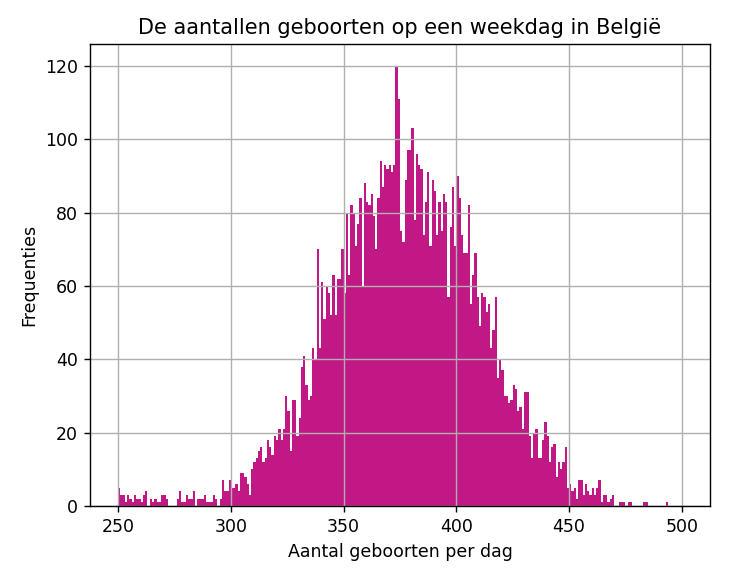
\includegraphics[width=7cm]{img/LOEP/geboorten4.jpg}
        \end{minipage}\hfill
        \begin{minipage}[t]{0.5\linewidth}
            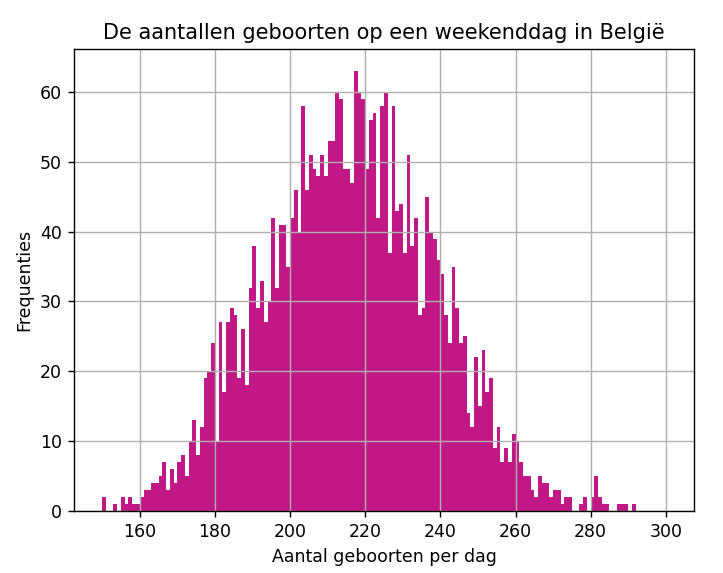
\includegraphics[width=7cm]{img/LOEP/geboorten6.jpg}
        \end{minipage}  }
        
    \antwoord{Beide frequentiediagrammen lijken normaalverdeelde klokvormen. Deze uitspraak is enkel op intuïtie gebaseerd. Om echt zeker te zijn van de normaliteit van de verdeling, moeten we bijkomend onderzoek doen.}

    \vraag{Laat het onderstaande Python-programma lopen en verklaar alle stappen. Je ziet nu het diagram van het aantal geboortes per dag tijdens de week (linkse afbeelding). Hoe pas je het programma aan om de andere grafiek te krijgen (rechtse afbeelding)?}

    \lstinputlisting[style=pythonstyle,linerange={1-24},firstnumber=1]{python/Aantalgeboortesperdag3.py}

    \antwoord{In regel 17 worden de weekdagen gedefinieerd in een \inline{array} met vijf woorden. Door de opsomming van de dagen te wijzigen, kun je overschakelen van het weekdiagram naar het weekenddiagram. Let op: voor het weekenddiagram moet ook de \inline{range} op de horizontale as aangepast woorden, zie regel 19. In regel 18 wordt het dataframe \inline{geboortes} beperkt tot het dataframe \inline{geboortesweek}. Dat gebeurt door het localiseren van de data met \inline{loc} en door de test \inline{isin} waarmee nagegaan wordt of een woord in een \inline{array} voorkomt. Regel 6 is in principe nog niet nodig. Alleen voor vergevorderde analyse, bijvoorbeeld voor de QQ-plots (zie verderop), is het pakket \inline{statsmodels} onontbeerlijk.}

    \vraag{Bereken via enkele extra regels in het Python-programma het gemiddelde (als schatter voor $\mu$) en de standaardafwijking (als schatter voor $\sigma$) van het aantal geboortes per dag bij de selectie van de geboortes op een weekdag.}
    \lstinputlisting[style=pythonstyle,linerange={25-32},firstnumber=25]{python/Aantalgeboortesperdag3.py}

    \antwoord{Het gemiddelde is $372,5$ en de standaardafwijking is $41,8$.}
    
    \vraag{Breid je programma nogmaals uit met de programmaregels hieronder. Bereken de kans dat het aantal geboortes per dag op een weekdag in het interval $[\mu-2\cdot\sigma,\mu+2\cdot\sigma]$ ligt. Bevestigt dit het vermoeden dat de aantallen geboortes tijdens weekdagen normaalverdeeld zijn? Wordt dit vermoeden ook bevestigd door de kansen te berekenen dat het aantal geboortes in het interval $[\mu-\sigma,\mu+\sigma]$ ligt? En wat concludeer je als je het interval $[\mu-3\cdot\sigma,\mu+3\cdot\sigma]$ onder de loep neemt?} 

    \lstinputlisting[style=pythonstyle,linerange={33-41},firstnumber=33]{python/Aantalgeboortesperdag3.py}
    
    \antwoord{De kans op een waarde in het interval $[\mu-2\cdot\sigma,\mu+2\cdot\sigma]$ is $0,95$. Dit versterkt het vermoeden van normaliteit. De kans op een waarde in $[\mu-3\cdot\sigma,\mu+3\cdot\sigma]$ is $0,97$. Ook deze waarde is in de buurt van de verwachtingen. De kans op een waarde in $[\mu-\sigma,\mu+\sigma]$ is $0,78$. Dit getal wijkt al wat meer af van de verwachte $0,68$. We vermoeden nu dat de geboortedata tijdens de week niet normaalverdeeld zijn.}

    \vraag{Doe dezelfde normaliteitstest voor de geboortedata tijdens het weekend. Wat concludeer je?}

    \antwoord{Nu stemmen de kansen bijna perfect overeen met de $68$-$95$-$99$-regel. We vermoeden dus dat de data normaalverdeeld zijn. Het blijft echter bij een vermoeden want deze data garanderen bijvoorbeeld niet dat de verdeling symmetrisch is, dat het histogram slechts één top heeft ... Statistici zijn hier niet voor honderd procent tevreden met het normaliteitsbewijs. Ze gebruiken hier liever een straffere controle, bijvoorbeeld de QQ-plot.}
    
\end{vraagenantwoord}
\end{lesactiviteit}
\begin{multicols}{2}

\subsection{De QQ-plot} 
Een van de meest gebruikte middelen om na te gaan of een variabele in een dataset normaal verdeeld is, is een QQ-plot. In de figuur hieronder zie je een QQ-plot voor de weekdata (links) en voor de weekenddata (rechts). In elk van beide figuren zie je een rode lijn en een reeks van blauwe punten. De blauwe punten zijn gebaseerd op de dataset, terwijl de rode lijn de kandidaat voor de normale verdeling weergeeft, namelijk die met verwachtingswaarde het gemiddelde \(\bar{x}\) van de dataset en als standaardafwijking de steekproefstandaardafwijking \(s\) van de dataset

Hiermee kunnen we op een visuele manier beoordelen hoe goed de dataset aansluit bij een normale verdeling. Als de gegevens uit onze dataset perfect normaal verdeeld zijn, dan moeten de blauwe punten op de rode rechte liggen. Deze QQ-plots versterken dus het vermoeden uit de vorige lesactiviteit: de weekdata zijn niet normaal verdeeld, de weekenddata zijn het wel.

\end{multicols}
        \begin{minipage}[t]{0.5\linewidth}
            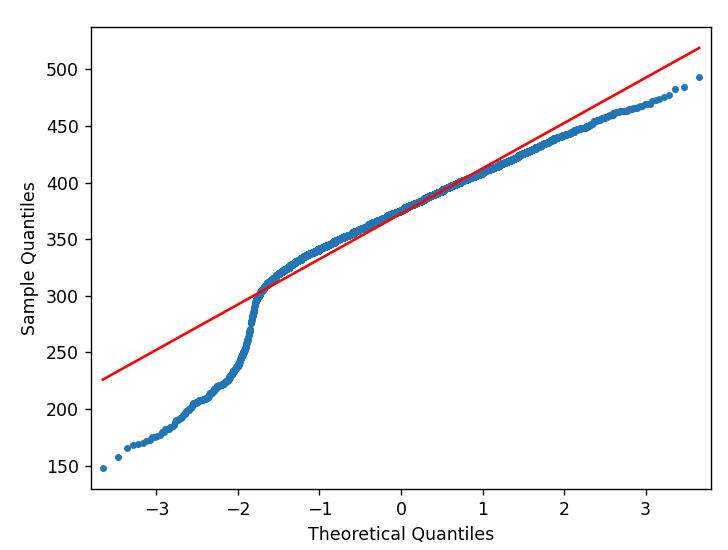
\includegraphics[width=7cm]{img/LOEP/geboorten5.jpg}
        \end{minipage}\hfill
        \begin{minipage}[t]{0.5\linewidth}
            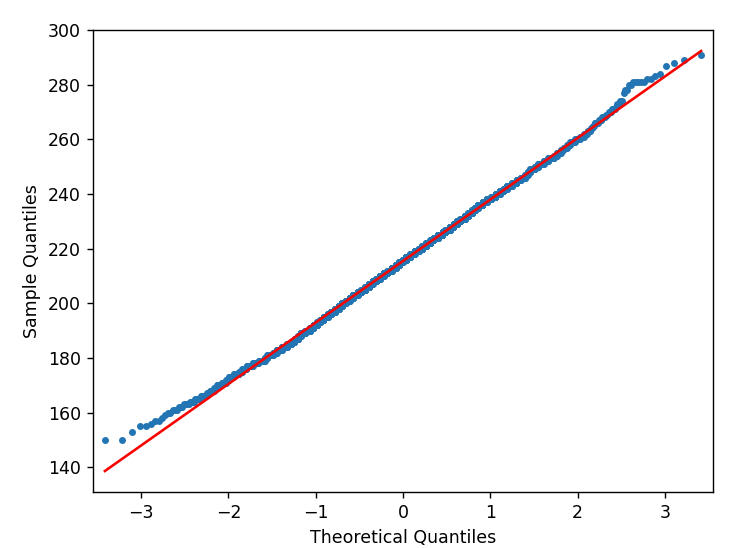
\includegraphics[width=7cm]{img/LOEP/geboorten7.jpg}
        \end{minipage}
        %\captionof{figure}{QQ-plot voor weekdagen (links) en weekenddagen (rechts)}
\begin{multicols}{2}

Focussen we nu even op de rode rechte op de QQ-plots. Die gaat door het punt $(0,\mu)$ en heeft richtingscoëfficiënt $\sigma$. Deze rechte ligt helemaal vast als de twee kengetallen ($\mu$ en $\sigma$) van de normale verdeling berekend zijn. Het is met deze referentierechte dat we de hele dataset zullen vergelijken. We illustreren de aansluiting van de blauwe QQ-plot met de rode referentierechte in de linkse figuur voor het $2,5\%$-kwantiel. 

Bij de standaardnormale verdeling ligt het $2,5\%$-kwantiel bij $-2$ d.w.z.\ dat $2,5\%$ van de meetwaarden links van $-2$ liggen. Het theoretische $2,5\%$-kwantiel van onze normaalverdeling ligt in de buurt van 290. Dat zie je als je naar het beeld van $-2$ door de rode referentiefunctie kijkt. De blauwe QQ-plot sluit helemaal niet aan bij deze refentierechte. Het beeld van $-2$ door de QQ-plot is ongeveer 220. Dit betekent dat het $2,5\%$-kwantiel van de reële geboorteaantallen veel lager ligt dan verwacht. Concreter: $2,5\%$ van de geboorteaantallen ligt lager dan 220 geboortes per dag. Waarden rond de 220 zijn helaas niet te zien op het histogram omdat we bij het tekenen van het histogram een minder geschikte \inline{range} gekozen hebben. Kan gebeuren ...

Een mogelijke verklaring voor het te lage $2,5\%$-kwantiel is te vinden in de te hoge frequenties in de lage regionen, bijvoorbeeld bij 220 geboortes per dag. Zulke uitschieters bij de weekdagen zijn te wijten aan weekdagen die mogelijk feestdagen zijn dag van de arbeid, Allerheiligen, paasmaandag, ... Op deze dagen worden bevallingen veelal on hold gezet. Als we de gegevens op feestdagen zouden kunnen wegfilteren, hebben we tijdens de week mogelijk wel een normale verdeling van de geboortecijfers.

We eindigen met een korte uitbreiding van het programma voor het maken van QQ-plots.

\end{multicols}
\afbeelding[12cm]{img/bevallingen.jpg}{}{}

\lstinputlisting[style=pythonstyle,linerange={42-46},firstnumber=42]{python/Aantalgeboortesperdag3.py}



\begin{multicols}{2}


        
        \section{Wat met ChatGPT en andere AI?}
        ChatGPT is, net zoals vele andere tekstgenererende artificiële intelligentie (AI), moeilijk weg te denken in het huidige leven. Leerlingen maken hier vaak al gebruik van voor schrijftaken, voor oefeningen \ldots{} Ook voor het produceren van pythoncodes kan dit ingezet worden en dat hoeft niet noodzakelijk slecht te zijn. Toch hebben we daar enkele praktische bedenkingen bij.

        Enerzijds is er weinig tot geen leerproces voor een leerling die alle codes laat schrijven door AI zonder er zelf bij na te denken. Het kan wel nuttig zijn om AI te raadplegen wanneer we niet weten hoe een bepaalde stap in het programma te schrijven of om inspiratie op te doen, maar het menselijk denkproces mag niet uitgeschakeld worden.

        Anderzijds is de door AI geproduceerde code niet altijd effici\"ent of overzichtelijk. Een mooi voorbeeld daarvan staat in de lesactiviteit over de Fibonacci-rij. De derde verbetering die daar aangeboden wordt, is van de hand van ChatGPT. We gebruikten de prompt: \begin{citaat}
            Schrijf een Python-programma dat de eerste \emph{10} getallen uit de rij van Fibonacci opslaat in een lijst en tenslotte de lijst print.
        \end{citaat}
        Hoewel deze code doet wat ze moet doen, is ze weinig inzichtelijk. Zo behoudt ChatGPT beide variabelen \inline{a} en \inline{b} doorheen de code, hetgeen niet echt logisch is bij het werken met een lijst. De menselijke code uit de vierde verbetering is in dat opzicht beter aangezien ze zowel korter is als minder variabelen gebruikt.

        We zijn er daarom van overtuigd dat het schrijven van pythoncode pas kan overgelaten worden aan ChatGPT als de codevrager ook begrijpt wat er staat en als hij de code kan opschonen en/of verbeteren.

\section{Technische slotopmerking} \label{sec:technisch}
Om een programma in Python te laten lopen (te runnen)  is het handig dat je gebruik maakt van een \emph{editor} of van een \emph{IDE} (Integrated development environment). 

\href{https://code.visualstudio.com/}{\emph{Visual Studio Code}} (VSC) is een gratis IDE die ruime mogelijkheden biedt. Hij werkt onder Windows, onder macOS en onder Linux. Je kunt deze IDE niet alleen gebruiken om Python-programma's te ontwikkelen maar ook voor JavaScript, C++, PHP ... in totaal voor meer dan 100 andere programmeertalen. 

\begin{center}
    
\includegraphics[width=0.4
    \linewidth]{img/LOEP/logo2.jpg}
    \captionof{figure}{Het logo van Visual Studio Code}
    \label{logo2}
\end{center}

VSC spoort syntactische fouten op, zoals het ontbreken van een rechterhaakje wanneer je alleen een linkerhaakje gezet hebt of het verwijzen naar een variabele waarvan je de waarde vergat in te stellen. Je kunt \emph{breakpoints} instellen om slechts een gedeelte van een programma te runnen. Je kunt een programma bovendien ook stap voor stap runnen en na elke stap de inhouden van de variabelen bekijken. Dit zijn goede hulpmiddelen bij foutdetectie. Handig is ook de tekstvoorspelling waarbij er suggesties gedaan worden voor woorden waarvan je het begin getypt hebt. En sinds kort kun je ook suggesties van AI opvragen.

Veelgebruikte bibliotheekprogramma's (packages) staan automatisch op je computer als je Python hebt geïnstalleerd (vanuit VSC). Minder frequent gebruikte bibliotheekprogramma's moet je eenmalig manueel downloaden. Zelf vonden we dit een heel gedoe. De makkelijkste manier is door gebruik te maken van PIP, de package installer van Python. Je zoekt best een filmpje op om te weten met welke instructie in de terminal je PIP aan het werk kunt zetten om de bibliotheekprogramma's te downloaden.


\begin{center}
    \includegraphics[width=0.4
    \linewidth]{img/LOEP/logo3.png}
    \captionof{figure}{Het logo van Thonny}
    \label{logo3}
\end{center} 

Een alternatief voor VSC is \href{https://thonny.org/}{\emph{Thonny}}. Thonny is een gratis programma dat gemaakt is door de Estse programmeur Aivar Annamaa. Het is een IDE die ontwikkeld is voor beginnende pythongebruikers. Andere programmeertalen kan Thonny niet aan. Ik moet toegeven dat het installeren van de bibliotheekprogramma's ook hier een bijzondere zorg was.

In onze school worden VSC en Thonny door elkaar gebruikt in de lessen informaticawetenschappen. Leerlingen die meer ervaring hebben in programmeren, kiezen vaak voor de eerste optie. Wie minder ervaring heeft, kiest vaak voor Thonny.

Uiteraard zijn er nog andere opties mogelijk om in de klas te werken met Python. Populair is onder andere de IDE \href{https://www.jetbrains.com/pycharm/}{\emph{Pycharm}}, ontwikkeld door de Tsjechische firma \emph{JetBrains}. Van Pycharm bestaat er een gratis versie en een betaalde versie. 



%Slotopmerking: we kunnen het hier kort hebben over het verschil tussen recursief en iteratief programmeren?
%\end{multicols}


%% LESACTIVITEIT %%%%%%%%%%%%%%%%%%%%%%%%%%%%%%%%%%%%%%%%%%%%%%%%%%%%%%%%%%%%%%%
%% Gebruik de {lesactiviteit} omgeving om een lesactiviteit aan te geven. Gebruik dit enkel BUITEN een multicols omgeving!
%\begin{lesactiviteit}{Titel van de lesactiviteit}
	
%	\begin{vraagenantwoord}
%		\vraag{\lipsum*[1][1-2]}
%		\antwoord{\lipsum*[1][3-4]}
		
%		\vraag{\lipsum*[1][1-2]}
%		\antwoord{\lipsum*[1][3-4]}
%	\end{vraagenantwoord}
	
%\end{lesactiviteit}
%\begin{multicols}
\end{multicols}

\stopcontents[inhoudloep]		% om inhoud voor het loep artikel te eindigen
\vspace{-1cm}

%% BRONNEN %%%%%%%%%%%%%%%%%%%%%%%%%%%%%%%%%%%%%%%%%%%%%%%%%%%%%%%%%%%%%%%%%%%%%
\begin{bronnen}
    \item Hautekiet, G., Moons, F. \& Van den Broeck L. (2022). Klaar voor de GRexit. \emph{Uitwiskeling 38/3}, 27-36.
    
    \item Deprez, J. \& Vanlommel, E. (2020). QQ-plots. \emph{Uitwiskeling 36/1}, 45-48.
    
    \item Labie, R. \& Stulens, K. (2005). \emph{Iteratie, dynamische processen en numerieke methoden} \url{https://www.uhasselt.be/media/rmolgsij/idn.pdf}

    \item Peeters, D., \emph{Tutorial Programmeren in Python}, UHasselt, \\ \href{https://www.uhasselt.be/nl/info-voor/aanbod-voor-scholen-en-onderwijsprofessionals/lesmateriaal/tutorial-programmeren-in-python}{https://www.uhasselt.be/nl/info-voor/aanbod-voor-scholen-en-onderwijsprofessionals/lesmateriaal/tuto\\rial-programmeren-in-python}

    \item Schrijvers, T. et al. (2021), \emph{eTeacher}, KU Leuven, \url{eteacher.be}
    \item Wikiwand. \emph{Approximations of $\pi$}. \url{https://www.wikiwand.com/en/articles/Approximations_of_%CF%80}

    \item Roelens, M., Op de Beeck, R \& Van Leemput, G. (1994). \emph{Toestellen voor wiskundelessen, catalogus bij de tentoonstelling voor 10 jaar Uitwiskeling}, 64-65.
    
    \url{programmeren-in-python}
    \item Van Renterghem, J. et al. \emph{Dodona, Leren programmeren voor secundair en hoger onderwijs}, UGent, \url{dodona.be}


\end{bronnen}